\documentclass[12pt]{article}
\usepackage{sbc-template}
\usepackage{graphicx,url}
\usepackage[utf8]{inputenc}
\usepackage[brazilian]{babel}
\usepackage{float}
\usepackage{array}
\usepackage{booktabs}
\usepackage[section]{placeins}
\usepackage{amsmath,amssymb}

\sloppy

\title{Predição de criminalidade contra pessoas trans e travestis: \\ Relação entre notificações de violência e indicadores municipais no Brasil}

\author{Ana Queiroz da Silva, Natália Metolina, Pedro Henrique Teixeira Soares}

\address{Escola de Artes, Ciências e Humanidades -- Universidade de São Paulo (USP)\\
Rua Arlindo Bétio nº 1000 -- São Paulo -- SP -- Brasil}

  
\begin{document}

\maketitle
     
\begin{abstract}
To give visibility to violence against transgender people and \textit{travestis}, this work combines 27,441 reports of violence against LGBT people made to the Disque 100 hotline (2011--2022) with municipal indicators to identify municipalities with alarming numbers and to predict waves of reports. After accounting for population size, 141 municipalities were alarming in 2020--2022, 83 of them with fewer than 100,000 inhabitants. In one-year-ahead forecasts, LightGBM reduced the error by 16.7\% (95\% CI: 13.3--20.3) relative to a population-only allocation and, monitoring 1\% of municipalities, captured 31\% of the waves. Reports were more frequent where there are more same-sex couples, higher density and a municipal human rights ombudsman, and waves did not spread to neighbouring cities. Transgender victims accounted for 18\% of reports with recorded identity and suffered more severe and public violence. The effect of the 2019 Supreme Court decision could not be measured, as recording changes dominated the series.
\end{abstract}

\begin{resumo}
Para dar visibilidade à violência contra pessoas trans e travestis, este trabalho combina 27.441 denúncias de violência contra pessoas LGBT feitas ao Disque 100 (2011--2022) com indicadores municipais para identificar municípios com números alarmantes e prever ondas de denúncias. Descontado o porte, 141 municípios foram alarmantes em 2020--2022, 83 deles com menos de 100 mil habitantes. Na previsão de um ano à frente, o LightGBM reduziu o erro em 16,7\% (IC 95\%: 13,3--20,3) em relação à distribuição pela população e, monitorando 1\% dos municípios, reuniu 31\% das ondas. Houve mais denúncias onde há mais casais do mesmo sexo, maior densidade e ouvidoria de direitos humanos, e as ondas não se espalharam para cidades vizinhas. As vítimas trans foram 18\% das denúncias com identidade registrada e sofreram violência mais grave e pública. Não foi possível medir o efeito da decisão do STF de 2019, pois mudanças no registro dominaram a série.

\textbf{Palavras-chave:} violência contra população trans; pessoas trans e travestis no Brasil; Disque 100; previsão espaço-temporal; aprendizado de máquina.
\end{resumo}


\section{Introdução}
\label{sec:introducao}

A produção de dados referentes à população trans no Brasil é um desafio persistente e uma limitação para a elaboração de políticas públicas. Os Censos elaborados pelo Instituto Brasileiro de Geografia e Estatística (IBGE) não apresentam dados especializados referentes à identidade de gênero. A população transgênera é definida como o conjunto de pessoas que se identificam com um gênero incongruente ou diferente daquele que lhes foi atribuído ao nascer e estima-se que representam entre 0,1\% e 2\% da população brasileira, a depender da localidade. Estima-se que o total da população transgênera no Brasil se distribua da seguinte forma: Norte 8\%, Nordeste 26\%, Centro-Oeste 7\%, Sudeste 44\% e Sul 15\% \cite{spizziri_eufrasio_lima:2021}. Travestis  são uma identidade de gênero revindicada na América Latina, reunindo pessoas designadas como do sexo masculino ao nascer, mas que se identificam com o feminino, embora não necessariamente se identifiquem como mulheres \cite{leal_silva_lizzi:2026}. Para fins de pesquisa abarcaremos as categorias "transgênero", "travesti" e "transexual", esta última presente em bases de dados e documentos oficiais dos programas de saúde públicos, atendendo as diversas fontes utilizadas no trabalho.

A violência é um fenômeno complexo e polissêmico, sendo delimitado neste trabalho às definições presentes na Classificação Internacional de Doenças, caracterizando-se pelo uso intencional da força ou poder que possa ocasionar lesão, morte, privação, deficiência ou dano psicológico \cite{marinho_tomazelli_firianelli:2024}. Em 2011 a notificação de violência autoprovocada e interpessoal integrou a lista de notificação compulsória e foi incluída no Sistema de Informação de Agravos de Notificação (Sinan) e em 2014, para contemplar a Política Nacional de Saúde Integral de Lésbicas, Gays, Bissexuais, Travestis e Transexuais, foram incluídas na ficha de notificação as variáveis “orientação sexual”, “identidade de gênero” e "nome social". Em 2019, o Supremo Tribunal Federal (STF) incluiu a transfobia nos crimes previstos na Lei do Racismo (Lei nº 7.716/1989). Dados produzidos e organizados por associações e ONGs nacionais e internacionais indicam o Brasil como líder nos índices de violência e mortalidade por crimes violentos decorrentes da transfobia. O Sinan e o DATASUS tornaram-se as principais fontes de dados para as análises acadêmicas. Uma fonte menos explorada é o Disque Direitos Humanos (Disque 100), que recebe, por telefone e outros canais, denúncias de violações de direitos humanos feitas pela própria vítima ou por terceiros, e que mantém desde 2011 um recorte específico para a população LGBT. Diferente do Sinan, que registra os casos que chegam a um serviço de saúde, o Disque 100 também capta violências que raramente geram atendimento, como a discriminação e a violência psicológica. Todas essas bases, no entanto, enfrentam um cenário de subnotificação e dificuldade de desagregação da população trans do conjunto da população LGBT+, não representando com fidelidade a realidade da violência contra trans e travestis no Brasil.

As políticas nacionais de saúde voltadas especificamente para a população trans, que exercem um papel fundamental no acolhimento institucional, começaram a ser estruturadas e ampliadas de forma mais consistente nas últimas décadas, tendo como marcos fundamentais o Processo Transexualizador, formalizado em 2008, a Política Nacional de Saúde Integral LGBT, instituída em 2011, e a portaria do Ministério da Saúde de 2009, que assegura o direito ao uso do nome social em atendimentos prestados na rede pública de saúde, conquista esta que posteriormente foi convertida em decreto federal no ano de 2016. O Processo Transexualizador, no entanto, ainda é um programa com pouca distribuição pelo território nacional, tendo atualmente 26 municípios no país, em sua maioria grandes centros urbanos, concentrando-se principalmente nas regiões Sudeste e Sul, seguidos do Nordeste.

A partir deste cenário, o trabalho parte da constatação de que crimes contra a população LGBT, e em especial contra pessoas trans e travestis, têm pouca visibilidade, e de que saber onde as denúncias são desproporcionalmente altas é um primeiro passo para direcionar essa atenção. O objetivo é identificar os municípios brasileiros com números alarmantes de denúncias de violência contra pessoas LGBT e, a partir das suas tendências e características, prever em quais cidades tendem a surgir ondas de denúncias. Como a amostra de vítimas trans é pequena, as análises sempre comparam esse grupo com o total da comunidade LGBT. Quatro perguntas guiam o trabalho: (i) onde estão e como se agrupam os municípios com números alarmantes; (ii) se indicadores municipais permitem prever ondas de denúncias e qual modelo o faz melhor; (iii) em que a violência contra pessoas trans difere da violência contra as demais pessoas LGBT, em proporção e em perfil; e (iv) se a inclusão da transfobia na Lei do Racismo pelo STF, em 2019, alterou o número de denúncias. Os fatores associados a mais denúncias mostram onde o registro funciona e onde ele falta. O reforço desses fatores pode ampliar a notificação da violência e, como consequência, tornar as bases de dados mais consistentes para a elaboração de políticas de prevenção de crimes que vitimam a população trans.

O resultado principal é que é possível antecipar onde as denúncias se concentram. O LightGBM foi o melhor modelo e, acompanhando poucos municípios, reúne uma parcela relevante das ondas; os fatores mais associados às denúncias são a visibilidade da população LGBT e a existência de canais institucionais. Por outro lado, as mudanças administrativas no Disque 100 impedem medir o efeito da decisão do STF. As seções seguintes apresentam os trabalhos correlatos (Seção~\ref{sec:correlatos}), a metodologia (Seção~\ref{sec:metodologia}), os resultados e sua discussão (Seção~\ref{sec:resultados}) e a conclusão (Seção~\ref{sec:conclusao}).


\section{Trabalhos Correlatos}
\label{sec:correlatos}

\subsection{Violência contra pessoas trans nas bases do SUS}

Leal et al. \cite{leal_silva_lizzi:2026} analisaram 45.715 notificações de violência contra pessoas trans no Sinan entre 2015 e 2023, com um modelo bayesiano hierárquico espaço-temporal de Poisson ajustado por INLA, tendo as 27 unidades da federação como unidade de análise. As vítimas eram sobretudo mulheres trans (65,3\%), jovens de 19 a 29 anos (36,1\%) e pardas (44,6\%), e a violência física foi a mais frequente (65,9\%). A taxa bruta de notificação subiu de 74,3 para 214,0 por 100 mil pessoas trans estimadas entre 2015 e 2023, com as maiores taxas no Sudeste e no Sul, incluindo Minas Gerais, e a autocorrelação espacial só foi significativa em 2023. O estudo mostra que a violência notificada não se distribui ao acaso no território, mas não desce ao nível municipal nem faz previsão.

Marinho Neto et al. \cite{marinho_tomazelli_firianelli:2024} estudaram as notificações de violência autoprovocada e interpessoal contra pessoas trans de 20 a 59 anos no Sinan, de 2015 a 2022, com o método de Prais-Winsten. As notificações trans foram 1,7\% do total e caíram no período, enquanto cresceram o número de municípios notificantes (45,8\%) e as violências autoprovocada e sexual. Os agressores eram majoritariamente homens com vínculo afetivo com a vítima, sobretudo no caso das mulheres trans (43,4\%). A análise descreve a tendência nacional, sem relacionar as notificações às características dos municípios.

Luis et al. \cite{luis:2025} parearam as notificações de violência contra pessoas trans no Sinan com os óbitos do Sistema de Informações sobre Mortalidade (SIM) de 2014 a 2022. Das 36.452 notificações, o pareamento recuperou 1.325 óbitos, dos quais 563 (42,5\%) por causas violentas. Um modelo de Poisson mostrou maior prevalência de morte violenta entre os mais jovens (razão de prevalência de 4,29 entre 10 e 14 anos), com registro de lesão autoprovocada (1,50), com agressão por arma de fogo (2,00) e quando o óbito ocorreu menos de seis meses após a notificação (2,07). O trabalho liga violência notificada e morte, mas no nível individual e com acesso a dados identificados.

Em conjunto, esses estudos indicam que as notificações ainda não representam a realidade da violência contra pessoas trans, pela subnotificação e pela dificuldade de separar essa população do conjunto LGBT, mas que o aumento de municípios notificantes amplia a visibilidade do problema.

\subsection{Aprendizado de máquina em notificações de violência}

Coelho et al. \cite{coelho_jiv:2025} usaram Prophet e Random Forest sobre 2.635.514 notificações de violência contra a mulher no Sinan (2013--2023), combinadas a dados do IBGE, e projetaram, a partir de um crescimento médio de 2,26\% ao ano, um aumento de cerca de 95\% até 2033. Lucca e Romero \cite{lucca_romero_sbbd:2026} compararam regressão logística regularizada, Random Forest e LightGBM em 2,22 milhões de notificações de violência contra a mulher (2018--2024), com divisão temporal entre treino e teste, para distinguir violência física, psicológica e sexual. Os modelos não lineares acrescentaram pouco ao linear, o balanceamento de classes prejudicou a calibração das probabilidades e 44,9\% dos casos de violência psicológica não foram identificados, o que os autores associam à subnotificação presente na própria base. Esses trabalhos mostram que algoritmos baseados em árvores de decisão extraem padrões de bases administrativas de violência, mas tratam o país como um todo ou classificam casos individuais, sem prever onde os casos vão se concentrar, e não foram aplicados à população LGBT (Tabela~\ref{tab:referencia}).

\begin{table}[!htb]
\centering
\caption{Síntese dos trabalhos correlatos e deste trabalho}
\label{tab:referencia}
{\renewcommand{\arraystretch}{1.15}\footnotesize
\begin{tabular}{>{\raggedright\arraybackslash}p{2.5cm} >{\raggedright\arraybackslash}p{3.1cm} >{\raggedright\arraybackslash}p{3.2cm} >{\raggedright\arraybackslash}p{4.4cm}}
\toprule
\textbf{Trabalho} & \textbf{Dados e período} & \textbf{Método} & \textbf{Resultado relevante} \\
\midrule
Leal et al. \cite{leal_silva_lizzi:2026} & Sinan, 2015--2023, 27 UFs & Bayesiano hierárquico (INLA) & Violência não aleatória no território; maiores taxas no Sudeste e no Sul \\
\addlinespace
Marinho Neto et al. \cite{marinho_tomazelli_firianelli:2024} & Sinan, 2015--2022 & Prais-Winsten & Trans são 1,7\% das notificações; aumento das violências sexual e autoprovocada \\
\addlinespace
Luis et al. \cite{luis:2025} & Sinan e SIM, 2014--2022 & Pareamento e Poisson & 42,5\% dos óbitos pareados por causa violenta; risco maior entre jovens \\
\addlinespace
Coelho et al. \cite{coelho_jiv:2025} & Sinan e IBGE, 2013--2023 (mulheres) & Prophet e Random Forest & Projeção de cerca de +95\% até 2033 \\
\addlinespace
Lucca e Romero \cite{lucca_romero_sbbd:2026} & Sinan, 2018--2024 (mulheres) & Logística, Random Forest e LightGBM & Não lineares acrescentam pouco; 44,9\% da violência psicológica não identificada \\
\midrule
\textbf{Este trabalho} & Disque 100, IBGE, MUNIC e SUS, 2011--2022, 5.565 municípios & Bayes empírico, Getis-Ord, endêmico-epidêmico, LightGBM, Extra Trees e série interrompida & Municípios alarmantes e previsão de ondas, comparando vítimas trans e LGBT \\
\bottomrule
\end{tabular}}
\end{table}

\subsection{Lacuna e posicionamento}

Os estudos com dados do SUS descrevem tendências e perfis da violência contra pessoas trans no país ou nos estados, e os estudos com aprendizado de máquina tratam da violência contra a mulher. Nenhum deles identifica, município a município, onde as denúncias de violência contra pessoas LGBT estão acima do esperado, nem testa se é possível antecipar onde surgirão ondas. Este trabalho aborda essa lacuna em quatro frentes. A \textbf{fonte}: o Disque 100 capta violências que raramente chegam ao serviço de saúde, como a psicológica e a discriminação, presentes na maioria das denúncias. A \textbf{escala}: todos os 5.565 municípios, combinados a indicadores como a proporção de domicílios com casais do mesmo sexo do Censo 2022, a melhor aproximação disponível da população LGBT visível. A \textbf{previsão}: os modelos são avaliados prevendo anos que não viram e comparados a regras simples. O \textbf{registro}: as mudanças de sistema do Disque 100 são tratadas explicitamente. Como fontes, populações e alvos diferem, a comparação com esses estudos é qualitativa: o objetivo não é superar seus números, e sim acrescentar a dimensão municipal e preditiva.


\section{Metodologia}
\label{sec:metodologia}

Este é um estudo ecológico: para cada um dos 5.565 municípios e cada ano de 2011 a 2022, reunimos as denúncias de violência contra pessoas LGBT e características do município. As quatro análises, cada uma com seu código, servem à mesma pergunta central: \textbf{onde a violência notificada é alarmante e quais cidades tendem a ter ondas de denúncias}.

\subsection{Coleta de dados}

\textbf{Denúncias.} A fonte é o Disque Direitos Humanos (Disque 100), da Ouvidoria Nacional de Direitos Humanos. Usamos as denúncias de janeiro de 2011 a dezembro de 2022 em que a vítima pertence ao grupo ``população LGBTQIA+'' (50.045 linhas). De cada denúncia usamos data, município, perfil da vítima, tipo de violação, local, relação com o agressor e, desde 2020, quem denunciou e por qual canal.

\textbf{Características dos municípios.} Os dados municipais vieram de fontes oficiais, baixados por um script para que a coleta seja reproduzível (Tabela~\ref{tab:fontes}): IBGE, pesquisa MUNIC, Atlas da Violência, Atlas do Desenvolvimento Humano e SUS. A localização de cada município definiu os seus 10 vizinhos mais próximos. As fontes não tiveram o mesmo peso (última coluna): o histórico do Disque 100 foi a informação que mais contribuiu para a previsão, e se destacaram os casais do mesmo sexo, que medem a população LGBT visível de cada cidade, a densidade, a cor ou raça e a ouvidoria de direitos humanos.

\begin{table}[!htb]
\centering
\caption{Fontes de dados, variáveis municipais e seu papel nos resultados}
\label{tab:fontes}
{\renewcommand{\arraystretch}{1.2}\small
\begin{tabular}{>{\raggedright\arraybackslash}p{4.4cm} >{\raggedright\arraybackslash}p{3.7cm} >{\raggedright\arraybackslash}p{1.9cm} >{\raggedright\arraybackslash}p{3.3cm}}
\toprule
\textbf{Variável} & \textbf{Fonte} & \textbf{Período} & \textbf{Papel nos resultados} \\
\midrule
Denúncias contra pessoas LGBT & Disque 100 & 2011--2022 & variável prevista; histórico é o principal preditor \\
Casais do mesmo sexo; densidade & IBGE, Censo 2022 & 2022 & fatores mais fortes (mais denúncias) \\
População residente & IBGE & 2011--2022 & base do valor esperado \\
Cor ou raça; 15 a 29 anos & IBGE, Censos 2010 e 2022 & 2010, 2022 & pretos e pardos: menos denúncias \\
Políticas de direitos humanos e LGBT & IBGE, MUNIC & 2014, 2019, 2023 & ouvidoria: mais denúncias \\
PIB, renda, Gini e homicídios & IBGE, Atlas DH, Atlas da Violência & 2010--2022 & sem efeito \\
Processo Transexualizador & SUS (SIA/SIH) & 2008--2026 & sem efeito \\
\bottomrule
\end{tabular}}
\end{table}

\subsection{Limpeza e Normalização dos Dados}

O sistema de registro do Disque 100 mudou três vezes no período (2011--2019, primeiro semestre de 2020 e a partir de julho de 2020), com colunas, categorias e até o significado de uma linha diferentes: no formato mais recente, cada linha é uma violação, e não uma denúncia. Removemos 561 linhas repetidas e agrupamos as linhas da mesma denúncia e vítima, chegando a \textbf{27.441 registros}. Unificamos as colunas equivalentes dos três formatos, reunimos respostas como ``não informado'' na categoria ``desconhecido'' e agrupamos as cerca de 240 descrições de violação em nove tipos. Entre julho de 2020 e junho de 2022 o formulário não permitia registrar a identidade trans; nesse intervalo ela foi tratada como desconhecida, e não como zero. Associamos 97,6\% dos registros ao código do município (2.070 municípios) e montamos o painel de municípios e anos, com zero onde não houve denúncia. Valores em dinheiro foram corrigidos para reais de 2022, dados censitários foram interpolados entre 2010 e 2022, e as sete perguntas comuns às edições da MUNIC formaram um índice de política LGBT de 0 a 4. Por fim, categorias viraram colunas de 0 e 1, e medidas muito desiguais entre municípios, como população e PIB, foram transformadas em logaritmo e padronizadas.

\subsection{Análise Estatística das Notificações de Violência e Correlação entre Variáveis}

Em 91\% das combinações de município e ano não há denúncia, o que exige modelos para contagens com muitos zeros, e o volume nacional varia por razões administrativas do Disque 100. Por isso, tratamos o total do país como dado e modelamos \textit{onde} as denúncias se concentram. Para cada município e ano calculamos um \textbf{valor esperado}: quantas denúncias ele teria se recebesse uma fatia do total nacional proporcional à sua população.

\textbf{Análise 1 --- municípios alarmantes e previsão de ondas.} Dividimos as denúncias observadas pelas esperadas (risco relativo) e usamos a \textbf{suavização bayesiana empírica} \cite{marshall:1991} para que uma única denúncia numa cidade pequena não gere falso alarme; é \textbf{alarmante} o município com mais de 95\% de chance de estar acima do esperado. A estatística de \textbf{Getis-Ord} \cite{getis_ord:1992} identifica aglomerados de municípios alarmantes. Para prever as denúncias do ano seguinte, comparamos três modelos: o \textbf{endêmico-epidêmico} \cite{held_hohle_hofmann:2005}, criado para vigilância de surtos, que separa o volume esperado em parte estrutural, inércia do próprio histórico e propagação a partir dos vizinhos; o \textbf{LightGBM} \cite{ke:2017}, algoritmo de aprendizado de máquina baseado em árvores de decisão; e o \textbf{Extra Trees} \cite{geurts:2006}, da família das florestas aleatórias. Eles foram comparados com três regras simples: distribuir as denúncias só pela população, repetir a fatia histórica da cidade e repetir o ano anterior. Uma \textbf{onda} é um ano com pelo menos 5 denúncias e pelo menos o dobro do esperado, e um município entra em \textbf{alerta} quando supera o limite que o modelo considerava plausível em 95\% dos casos \cite{farrington:1996}. A confiabilidade do LightGBM foi verificada com curvas de aprendizado, \textit{bootstrap}, ablação, variação de parâmetros e valores SHAP.

\textbf{Análises 2 e 3 --- vítimas trans.} Uma \textbf{regressão binomial} mostra quais características do município se associam a uma proporção maior de vítimas trans entre as denúncias LGBT, comparando municípios dentro do mesmo ano. Uma \textbf{regressão logística}, conferida com o LightGBM, mostra quais características da denúncia tornam mais provável que a vítima seja trans (16.467 registros com identidade conhecida).

\textbf{Análise 4 --- decisão do STF.} Uma \textbf{série temporal interrompida} \cite{bernal:2017} compara as denúncias mensais após junho de 2019 com a tendência anterior, descontando pandemia, trocas de sistema e sazonalidade. No \textbf{teste de placebo}, repetimos a análise para cada mês de 2018 e 2019: se outro mês explicar melhor a mudança, ela não pode ser atribuída à decisão.

Os resultados são dados como \textbf{razão de taxas} (RR; 1,20 = 20\% mais denúncias que o esperado) ou \textbf{razão de chances}; se o IC 95\% inclui o 1, não há evidência de efeito. 

\subsection{Protocolo de validação, métricas e reprodução}

A avaliação simula o uso real. Em cada rodada, os modelos aprendem com todos os anos anteriores ao previsto e preveem os 5.565 municípios do ano seguinte, sem nenhum ajuste com o ano de teste (Tabela~\ref{tab:rodadas}). O LightGBM usa perda Tweedie (potência 1,3), própria para contagens com muitos zeros, taxa de aprendizado 0,03, 15 folhas, mínimo de 60 observações por folha e o log do valor esperado como termo fixo; o número de árvores vem da parada antecipada (até 2.000, parando após 100 sem melhora no último ano de treino), e o modelo é então retreinado com todos os anos. O Extra Trees usa 300 árvores, critério de Poisson e mínimo de 20 observações por folha; o endêmico-epidêmico é estimado por máxima verossimilhança. A semente é 42 em todos.

\begin{table}[!htb]
\centering
\caption{Rodadas da validação temporal: cada linha treina com os anos anteriores e prevê o ano indicado}
\label{tab:rodadas}
{\renewcommand{\arraystretch}{1.0}\footnotesize
\begin{tabular}{c c r r r r}
\toprule
\textbf{Ano previsto} & \textbf{Anos de treino} & \textbf{Obs. de treino} & \textbf{Sem denúncia} & \textbf{Ondas} & \textbf{Árvores} \\
\midrule
2016 & 2012--2015 & 22.260 & 92,7\% & 56 & 155 \\
2017 & 2012--2016 & 27.825 & 91,3\% & 59 & 130 \\
2018 & 2012--2017 & 33.390 & 92,5\% & 42 & 139 \\
2019 & 2012--2018 & 38.955 & 94,2\% & 42 & 352 \\
2020 & 2012--2019 & 44.520 & 93,4\% & 50 & 131 \\
2021 & 2012--2020 & 50.085 & 93,8\% & 31 & 942 \\
2022 & 2012--2021 & 55.650 & 85,8\% & 52 & 757 \\
\bottomrule
\multicolumn{6}{p{12.5cm}}{\footnotesize 5.565 municípios por ano previsto. Sem denúncia: municípios com zero registro. Árvores: escolhidas pela parada antecipada do LightGBM.}
\end{tabular}}
\end{table}

A métrica principal é o desvio de Poisson médio, que mede o erro de contagens sem deixar que as grandes cidades dominem a avaliação, como aconteceria com o erro quadrático; o ganho de cada modelo é a redução desse desvio em relação à referência ``só população''. Como as ondas são raras (menos de 1\% dos municípios por ano), elas são avaliadas pela precisão entre as 20 cidades apontadas como mais prováveis e pela precisão média, mais informativas que a acurácia em classes raras \cite{saito_rehmsmeier:2015}. Todas as fontes são baixadas por script e cada análise tem um código próprio, em Python 3.13 com \textit{statsmodels} 0.15, \textit{scikit-learn} 1.9, \textit{LightGBM} 4.7, \textit{SHAP} e \textit{PySAL}; com a semente fixa, repetir a execução reproduz os mesmos resultados.


\section{Resultados e Discussão dos Resultados}
\label{sec:resultados}

\subsection{Panorama das notificações}

Entre 2011 e 2022, o Disque 100 recebeu 27.441 registros de violência contra pessoas LGBT, vindos de 2.070 municípios. A maioria das vítimas era do gênero masculino (62\%), homossexual (68\%) e jovem (47\% entre 18 e 29 anos); em 28\% dos casos a raça/cor não foi informada. A violência psicológica esteve presente em 79\% dos registros, seguida da discriminação (53\%) e da agressão física (32\%). Desde 2020, 70\% das denúncias foram feitas pela própria vítima, quase todas por telefone.

As grandes variações no total nacional coincidem com mudanças administrativas, e não com mudanças conhecidas na violência (Figura~\ref{fig:serie}): o volume caiu após a troca de sistema em julho de 2020 e se multiplicou por cerca de 4,5 com o novo formulário de julho de 2022. Por isso, as análises olham para a \textit{distribuição} das denúncias entre as cidades, e não para o total do país.

\begin{figure}[!htb]
\centering
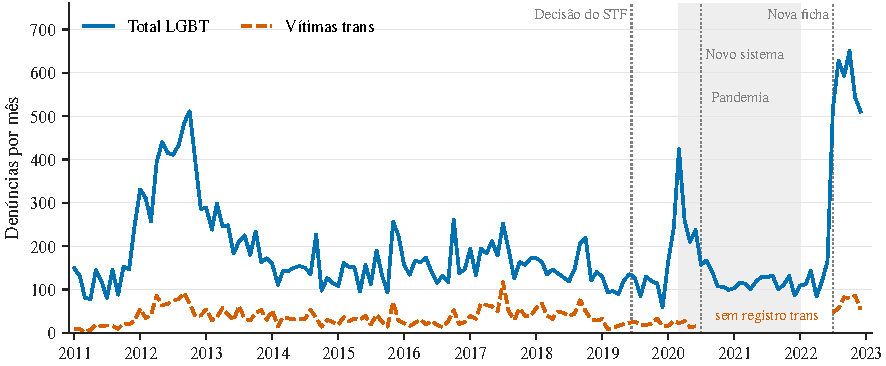
\includegraphics[width=\textwidth]{figuras/fig1_serie_mensal.pdf}
\caption{Denúncias mensais de violência contra pessoas LGBT (linha contínua azul) e contra vítimas trans (linha tracejada vermelha), 2011--2022. As linhas verticais pontilhadas marcam a decisão do STF e as mudanças no sistema de registro; a faixa cinza, a pandemia. Fonte: Disque 100 (ONDH/MDHC).}
\label{fig:serie}
\end{figure}

\subsection{Municípios com números alarmantes}

As denúncias se concentram: as 50 cidades com mais registros somam metade do total. Mas muitas denúncias não significam alto risco: São Paulo tem o maior número absoluto e fica apenas 31\% acima do esperado para o seu porte. Descontados o tamanho da população e o acaso, \textbf{141 municípios tiveram números alarmantes em 2020--2022}, 83 deles com menos de 100 mil habitantes. Os extremos foram Ubaporanga (MG, quase 30 vezes o esperado), Itaporanga (PB, 25), Cabo Frio (RJ, 17), Barbacena (MG, 10) e Campos dos Goytacazes (RJ, 8). Esses municípios formam \textbf{61 aglomerados de alto risco} na Zona da Mata e no Sul de Minas Gerais, na região metropolitana do Rio de Janeiro, no interior de São Paulo, em Goiás e no entorno de João Pessoa (Figura~\ref{fig:mapa}). Entre as 136 cidades com pelo menos 30 registros, 18 cresceram mais rápido que o total nacional, como Juazeiro (BA), Itaporanga (PB) e Barbacena (MG).

\begin{figure}[!htb]
\centering
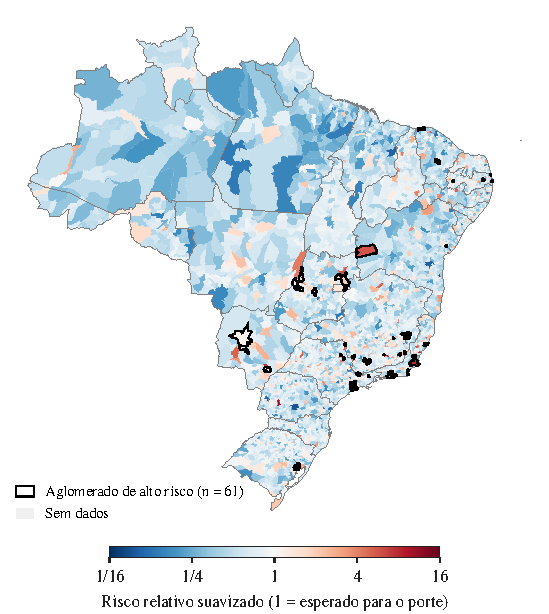
\includegraphics[width=0.62\textwidth]{figuras/fig3_mapa_risco.pdf}
\caption{Risco relativo suavizado de denúncias por município, 2020--2022. Vermelho: mais denúncias do que o esperado para o porte; azul: menos; branco: o esperado. O contorno preto marca os aglomerados de alto risco (Getis-Ord, $p<0{,}05$). Fonte: Disque 100 e IBGE.}
\label{fig:mapa}
\end{figure}

\subsection{Previsão de ondas e fatores associados}

\textbf{É possível prever.} Os três modelos previram melhor do que distribuir as denúncias só pela população, e as regras simples foram piores (Tabela~\ref{tab:validacao}). O LightGBM teve o melhor resultado, com erro 16,7\% menor que a referência, seguido pelo modelo endêmico-epidêmico (14,6\%). Repetir o ano anterior foi a pior estratégia: o número de denúncias de uma cidade varia muito de um ano para o outro, e o passado só ajuda combinado com as características do município. O ganho mais importante está nas ondas: das 20 cidades que o LightGBM apontou a cada ano como mais prováveis de ter uma onda, 37\% de fato a tiveram, contra 15\% usando só a população. Para dimensionar esse acerto: só cerca de 47 dos 5.565 municípios têm uma onda a cada ano (0,85\%), de modo que apontar 20 cidades ao acaso acertaria menos de 1\%, e o modelo acerta mais de 40 vezes isso. O acerto fica longe de 100\% porque a maioria das ondas é passageira e depende de quem denuncia; por isso, o modelo serve para priorizar a atenção, e não para emitir alarmes certeiros.

\begin{table}[!htb]
\centering
\caption{Desempenho dos modelos na previsão um ano à frente (média de 2016 a 2022)}
\label{tab:validacao}
{\renewcommand{\arraystretch}{1.2}\small
\begin{tabular}{p{4.6cm} p{2.6cm} p{2.6cm} p{3.0cm}}
\toprule
\textbf{Modelo} & \textbf{Redução do erro em relação à população} & \textbf{Acerto das 50 maiores cidades} & \textbf{Acerto entre as 20 cidades apontadas para onda} \\
\midrule
LightGBM & 16,7\% & 66\% & 37\% \\
Endêmico-epidêmico & 14,6\% & 63\% & 31\% \\
Extra Trees & 11,3\% & 63\% & 31\% \\
Só população (referência) & -- & 63\% & 15\% \\
Fatia histórica da cidade & $-$14,7\% & 61\% & 29\% \\
Repetir o ano anterior & $-$35,8\% & 55\% & 26\% \\
\bottomrule
\end{tabular}}
\end{table}

\textbf{O que está associado a mais denúncias.} O fator mais forte foi a proporção de domicílios com casais do mesmo sexo, a melhor medida disponível da população LGBT visível: municípios um pouco acima da média nesse indicador têm 13\% mais denúncias (Tabela~\ref{tab:coef}). A densidade teve efeito parecido, e a ouvidoria municipal de direitos humanos se associou a 23\% mais denúncias, sugerindo que um canal institucional facilita a denúncia. Municípios com mais pretos e pardos denunciaram 8\% menos, e Norte e Sul denunciaram menos que o Sudeste. Renda, PIB, desigualdade, homicídios, índice de política LGBT e Processo Transexualizador não mostraram relação com o volume de denúncias.

\begin{table}[!htb]
\centering
\caption{Características associadas a mais (RR $>$ 1) ou menos (RR $<$ 1) denúncias do que o esperado para o porte do município}
\label{tab:coef}
{\renewcommand{\arraystretch}{1.15}\small
\begin{tabular}{p{6.8cm} c c c}
\toprule
\textbf{Característica} & \textbf{RR} & \textbf{IC 95\%} & \textbf{Há efeito?} \\
\midrule
Casais do mesmo sexo (por desvio-padrão) & 1,13 & 1,08--1,18 & sim \\
Densidade demográfica (por desvio-padrão) & 1,12 & 1,07--1,18 & sim \\
População (por desvio-padrão) & 1,08 & 1,02--1,15 & sim \\
Pretos e pardos (por desvio-padrão) & 0,92 & 0,86--0,98 & sim \\
Tem ouvidoria de direitos humanos & 1,23 & 1,10--1,37 & sim \\
Região Centro-Oeste (em relação ao Sudeste) & 1,36 & 1,17--1,57 & sim \\
Região Sul & 0,72 & 0,64--0,81 & sim \\
Região Norte & 0,58 & 0,48--0,70 & sim \\
Renda domiciliar por pessoa & 1,01 & 0,92--1,10 & não \\
Taxa de homicídios no ano anterior & 0,99 & 0,94--1,03 & não \\
Índice de política LGBT (MUNIC) & 0,99 & 0,96--1,01 & não \\
Processo Transexualizador ativo & 0,71 & 0,34--1,46 & não \\
\bottomrule
\multicolumn{4}{p{12cm}}{\footnotesize Modelo endêmico-epidêmico, 2012--2022. Também incluídos, sem efeito: PIB por pessoa, Gini, população de 15 a 29 anos, estrutura municipal de direitos humanos, capital e Nordeste.}
\end{tabular}}
\end{table}

\textbf{As ondas são locais.} Das denúncias esperadas pelo modelo endêmico-epidêmico, 74\% vêm das características do próprio município, 26\% da inércia do seu histórico e apenas 0,3\% das cidades vizinhas: as ondas nascem e permanecem locais. A cada ano, entre 22 e 52 municípios entraram em alerta, e uma cidade em alerta tem quase 6 vezes mais chance de voltar a ficar em alerta no ano seguinte. Supondo para 2023 o mesmo volume nacional de 2022, a maior chance de onda foi estimada para Barbacena (MG, 40\%).

\subsection{Por que confiar na previsão}

O LightGBM constrói árvores de decisão uma a uma, cada nova árvore corrigindo os erros das anteriores. Nas curvas de aprendizado (Figura~\ref{fig:curvas}), o erro no treino cai continuamente, mas o erro no ano reservado para conferência cai até um ponto mínimo e depois volta a subir (até 11\% acima do mínimo): o treino é interrompido nesse ponto, o que impede que o modelo memorize o passado.

\begin{figure}[!htb]
\centering
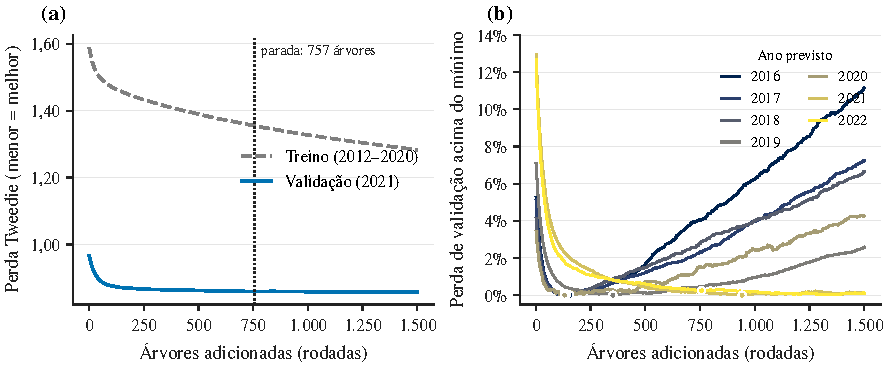
\includegraphics[width=\textwidth]{figuras/fig5_curvas_aprendizado.pdf}
\caption{Aprendizado do LightGBM ao longo das árvores. (a) Previsão de 2022: erro no treino (cinza tracejado) e no ano reservado para conferência (azul); a linha pontilhada marca onde o treino parou. (b) Erro de conferência acima do seu mínimo, para cada ano previsto; os círculos marcam o ponto de parada. Fonte: Disque 100 e IBGE.}
\label{fig:curvas}
\end{figure}

Reamostrando os municípios 2.000 vezes, a redução do erro ficou entre 13,3\% e 20,3\% (IC 95\%). O modelo foi melhor que a referência populacional em todos os sete anos testados e melhor que o endêmico-epidêmico em seis, e o ganho ficou entre 15,7\% e 17,3\% com diferentes parâmetros. Treinado só com as características dos municípios ou só com o histórico, ele já reduz o erro em cerca de 14\%; os vizinhos acrescentam apenas 0,15 ponto, o que confirma que as ondas não se propagam. As previsões são calibradas (o modelo previu 96\% das denúncias que ocorreram) e úteis para priorizar: monitorando só 1\% dos municípios por ano, os escolhidos pelo LightGBM concentram 31\% das ondas, contra 22\% pela população (Figura~\ref{fig:calib}). Por fim, os valores SHAP mostram que o modelo, sem nenhuma hipótese prévia, aprendeu as mesmas relações da Tabela~\ref{tab:coef}: histórico acima do esperado, mais casais do mesmo sexo e maior densidade elevam a previsão. A ablação e o SHAP estão detalhados no relatório técnico que acompanha os códigos.

\begin{figure}[!htb]
\centering
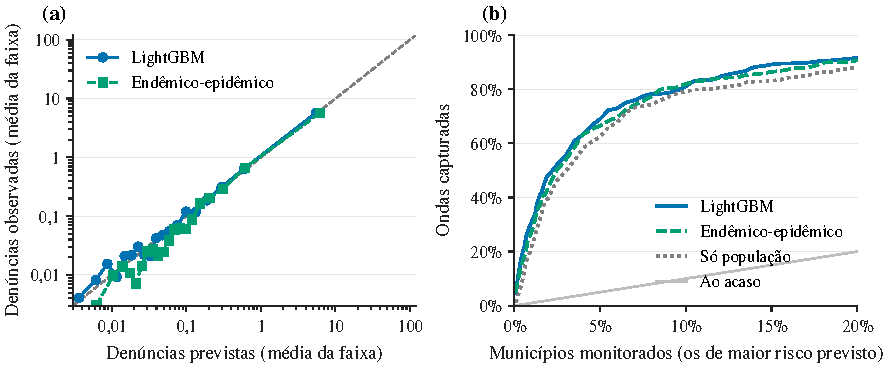
\includegraphics[width=\textwidth]{figuras/fig8_calibracao_captura.pdf}
\caption{(a) Calibração: denúncias previstas e observadas, por faixa de previsão (escala log); a linha tracejada indica previsão perfeita. (b) Percentual das 332 ondas de 2016 a 2022 capturado quando se monitoram os municípios de maior risco previsto; a linha cinza indica a escolha ao acaso. Previsões fora da amostra. Fonte: Disque 100 e IBGE.}
\label{fig:calib}
\end{figure}

\subsection{Violência contra pessoas trans e a decisão do STF}

\textbf{Proporção.} Nos períodos em que a identidade de gênero podia ser registrada, 18\% das denúncias LGBT tinham vítima trans (4.406 de 24.151). Comparando municípios no mesmo ano, essa proporção foi maior no Nordeste (chance 54\% maior que no Sudeste) e menor em cidades mais densas e com mais pretos e pardos. Os municípios alarmantes não diferem dos demais (17\% contra 19\%): as ondas atingem a comunidade LGBT como um todo.

\textbf{Perfil.} A violência contra pessoas trans é mais grave e mais pública (Figura~\ref{fig:perfil}). Em violações contra a vida, a chance de a vítima ser trans é 3 vezes maior, e também é maior na violência sexual (1,7) e física (1,4), na rua, e quando o agressor é desconhecido (1,7) ou profissional e agente de instituição (2,3). Esses registros são também mais incompletos: a raça/cor falta em 30\% deles, contra 16\% nos demais. O modelo distingue os dois grupos de forma moderada (AUC de 0,71), e o LightGBM não foi melhor que a regressão logística.

\begin{figure}[!htb]
\centering
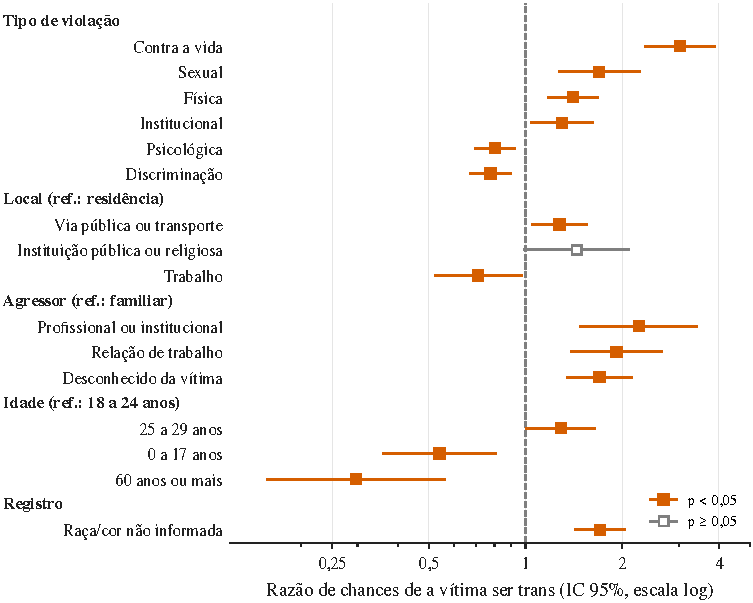
\includegraphics[width=0.85\textwidth]{figuras/fig4_perfil_trans.pdf}
\caption{Quanto cada característica da denúncia aumenta (à direita de 1) ou reduz (à esquerda de 1) a chance de a vítima ser trans. Quadrados cheios: efeito estatisticamente significativo ($p<0{,}05$); quadrados vazados em cinza: sem efeito. As linhas horizontais mostram o intervalo de confiança de 95\%. Fonte: Disque 100 (ONDH/MDHC).}
\label{fig:perfil}
\end{figure}

\textbf{Decisão do STF.} O STF incluiu a transfobia na Lei do Racismo em 13 de junho de 2019. O total de denúncias LGBT não mudou depois da decisão (RR 0,98; IC 95\%: 0,67--1,43). As denúncias com vítima trans caíram 48\%, mas o teste de placebo mostrou que a queda começou em fevereiro de 2019, quatro meses antes, junto com uma mudança no registro da categoria ``travesti''. Com só 13 meses de registros trans após a decisão, não é possível medir o seu efeito. As mudanças administrativas, por outro lado, pesaram muito: a troca de sistema reduziu o volume em 59\%, e o novo formulário o multiplicou por 4,5.


\subsection{Relação com a literatura, custo e limitações}

\textbf{Relação com a literatura.} A fatia de vítimas trans no Disque 100 (18\% das denúncias LGBT) é muito maior que a do Sinan, em que pessoas trans são 1,7\% de todas as notificações de violência \cite{marinho_tomazelli_firianelli:2024}. Os denominadores são diferentes e os números não são diretamente comparáveis, mas indicam que, entre as vítimas LGBT, as pessoas trans têm peso expressivo. O perfil converge: no Sinan predominam mulheres trans jovens, a violência física e o aumento da violência sexual \cite{leal_silva_lizzi:2026,marinho_tomazelli_firianelli:2024}, e aqui as vítimas trans são mais jovens e têm mais chance de sofrer violência física, sexual e contra a vida, em linha com a maior mortalidade violenta de pessoas trans jovens \cite{luis:2025}. A diferença está no agressor: no Sinan sobressaem parceiros com vínculo afetivo \cite{marinho_tomazelli_firianelli:2024}, enquanto no Disque 100 as vítimas trans se distinguem das demais vítimas LGBT pela violência de desconhecidos e de agentes de instituições, o que pode refletir o tipo de caso que cada canal recebe. No território, Leal et al. \cite{leal_silva_lizzi:2026} encontraram as maiores taxas no Sudeste e no Sul, com Minas Gerais entre os estados mais altos, e autocorrelação espacial fraca; os aglomerados em Minas Gerais e a contribuição quase nula dos vizinhos confirmam esse quadro no nível municipal. Como Lucca e Romero \cite{lucca_romero_sbbd:2026}, observamos que o aprendizado de máquina não supera a regressão logística ao classificar casos individuais (Análise 3); na previsão de contagens municipais com histórico, porém, o LightGBM superou o modelo estatístico. Diferente de Coelho et al. \cite{coelho_jiv:2025}, não projetamos o volume nacional, porque no Disque 100 ele depende de mudanças administrativas.

\textbf{Custo computacional.} As análises rodam em um computador comum, sem placa de vídeo. Cada rodada de treino levou de 0,5 a 4 segundos no LightGBM, de 2 a 4,5 segundos no endêmico-epidêmico e de 2,5 a 6,5 segundos no Extra Trees; a Análise 1 completa leva cerca de 1,5 minuto, e as verificações de confiabilidade, cerca de 4 minutos. O modelo mais preciso foi também o mais rápido.

\textbf{Limitações.} As conclusões têm seis limitações principais. Primeiro, o Disque 100 mede denúncias, e não a violência em si, e a subnotificação pode variar entre municípios. Segundo, o estudo é ecológico: as associações valem para municípios, e não para pessoas, e não indicam causalidade. Terceiro, a identidade trans não foi registrada entre julho de 2020 e junho de 2022, e há apenas 13 meses de registro trans após a decisão do STF. Quarto, a proporção de casais do mesmo sexo só existe no Censo de 2022, e outras variáveis censitárias foram interpoladas entre 2010 e 2022. Quinto, a previsão trata o volume nacional do ano seguinte como conhecido, pois ele depende de decisões administrativas que os modelos não antecipam. Sexto, os dados terminam em 2022, e as estimativas para 2023 ainda não foram conferidas.


\section{Conclusão}
\label{sec:conclusao}

É possível localizar os municípios em que a violência contra pessoas LGBT é denunciada muito acima do esperado e antecipar onde tendem a surgir ondas. Os 141 municípios alarmantes não são só grandes centros e se agrupam em regiões; o LightGBM foi o melhor modelo e, monitorando 1\% dos municípios, reúne quase um terço das ondas. Denuncia-se mais onde a população LGBT é mais visível, em cidades densas e onde há ouvidoria, e menos no Norte, no Sul e onde há mais pessoas pretas e pardas, o que é compatível com subnotificação, sem que os dados permitam separar menos violência de menos denúncia. As ondas são locais e persistentes. As vítimas trans são 18\% das denúncias, mas sofrem violência mais grave e pública, inclusive por agentes de instituições, e seus registros são os mais incompletos. Não foi possível medir efeito da decisão do STF: mudanças no registro pesaram mais que o marco legal. Como trabalhos futuros, propomos manter um campo estável de identidade de gênero no Disque 100, cruzar as denúncias com o Sinan e o SIM e testar a previsão com os dados de 2023 em diante.


\bibliographystyle{sbc}
\bibliography{sbc-template,referencias_metodo}

\end{document}
